\section{Research Frontiers}

GANs are a relatively new method, with many research directions still
remaining open.

\subsection{Non-convergence}

The largest problem facing GANs that researchers should try to resolve is the issue
of non-convergence.

Most deep models are trained using an optimization algorithm that seeks out a low
value of a cost function.
While many problems can interfere with optimization, optimization algorithms usually
make reliable downhill progress.
GANs require finding the equilibrium to a game with two players.
Even if each player successfully moves downhill on that player's update,
the same update might move the other player uphill.
Sometimes the two players eventually reach an equilibrium, but in other scenarios
they repeatedly undo each others' progress without arriving anywhere useful.
This is a general problem with games not unique to GANs, so a general solution
to this problem would have wide-reaching applications.

To gain some intuition for how gradient descent performs when applied to games
rather than optimization, the reader is encouraged to solve the exercise in
\secref{sec:xy_exercise} and review its solution in \secref{sec:xy_soln} now.

Simultaneous gradient descent converges for some games but not all of them.

In the case of the minimax GAN game (\secref{sec:minimax}),
\citet{Goodfellow-et-al-NIPS2014-small} showed that simultaneous gradient
descent converges {\em if the updates are made in function space}.
In practice, the updates are made in parameter space, so the convexity
properties that the proof relies on do not apply.
Currently, there is neither a theoretical argument that GAN games should
converge when the updates are made to parameters of deep neural networks,
nor a theoretical argument that the games should not converge.

In practice, GANs often seem to oscillate, somewhat like what happens in
the toy example in \secref{sec:xy_soln}, meaning that they progress from
generating one kind of sample to generating another kind of sample without
eventually reaching an equilibrium.

Probably the most common form of harmful non-convergence encountered in the GAN
game is mode collapse.

\subsubsection{Mode collapse}
\label{sec:mode_collapse}

Mode collapse, also known as \newterm{the Helvetica scenario}, is a problem that occurs
when the generator learns to map several different input $\vz$ values to the same output
point.
In practice, complete mode collapse is rare, but partial mode collapse is common.
Partial mode collapse refers to scenarios in which the
generator makes multiple images that contain the same color or texture themes,
or multiple images containing different views of the same dog.
The mode collapse problem is illustrated in \figref{fig:mode_collapse}.

Mode collapse may arise because the maximin solution to the GAN game is different
from the minimax solution.
When we find the model
\[ G^* = \min_G \max_D V(G,D), \]
$G^*$ draws samples from the data distribution.
When we exchange the order of the min and max and find
\[ G^* = \max_D \min_G V(G, D), \]
the minimization with respect to the generator now lies in the inner
loop of the optimization procedure.
The generator is thus asked to map every $\vz$ value to the single $\vx$
coordinate that the discriminator believes is most likely to be real rather than fake.
Simultaneous gradient descent does not clearly privilege $\min \max$ over $\max \min$
or vice versa. We use it in the hope that it will behave like $\min \max$ but it
often behaves like $\max \min$.


\begin{figure}
\centering
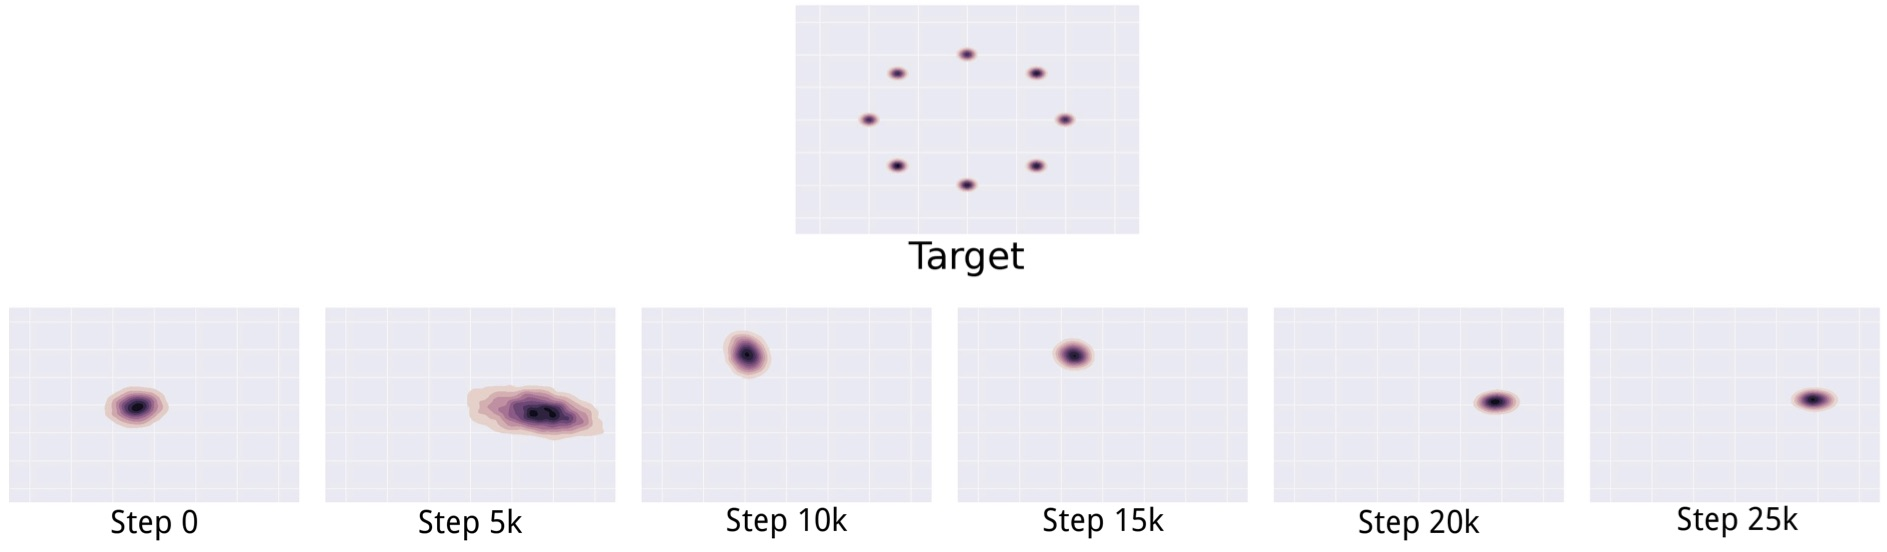
\includegraphics[width=\figwidth]{mode_collapse}
\caption{
An illustration of the mode collapse problem on a two-dimensional toy dataset.
In the top row, we see the target distribution $\pdata$ that the model should
learn. It is a mixture of Gaussians in a two-dimensional space.
In the lower row, we see a series of different distributions learned over time
as the GAN is trained.
Rather than converging to a distribution containing all of the modes in the
training set, the generator only ever produces a single mode at a time, cycling
between different modes as the discriminator learns to reject each one.
Images from \citet{metz2016unrolled}.
}
\label{fig:mode_collapse}
\end{figure}

As discussed in \secref{sec:which_divergence}, mode collapse does not seem to be
caused by any particular cost function.
It is commonly asserted that mode collapse is caused by the use of Jensen-Shannon
divergence, but this does not seem to be the case, because GANs that minimize
approximations of $\KL(\pdata \Vert \pmodel)$ face the same issues, and because
the generator often collapses to even fewer modes than would be preferred by the
Jensen-Shannon divergence.

Because of the mode collapse problem, applications of GANs are often limited to
problems where it is acceptable for the model to produce a small number of 
distinct outputs, usually tasks where the goal is to map some input to one of
many acceptable outputs.
As long as the GAN is able to find a small number of these acceptable outputs,
it is useful.
One example is text-to-image synthesis, in which the input is a caption for an
image, and the output is an image matching that description.
See \figref{fig:text2im} for a demonstration of this task.
In very recent work, \citet{reedgenerating} have shown that other models have
higher output diversity than GANs for such tasks (\figref{fig:low_diversity}),
but StackGANs \citep{zhang2016stackgan} seem to have higher output diversity than previous GAN-based
approaches (\figref{fig:stackgan}).


\begin{figure}
\centering
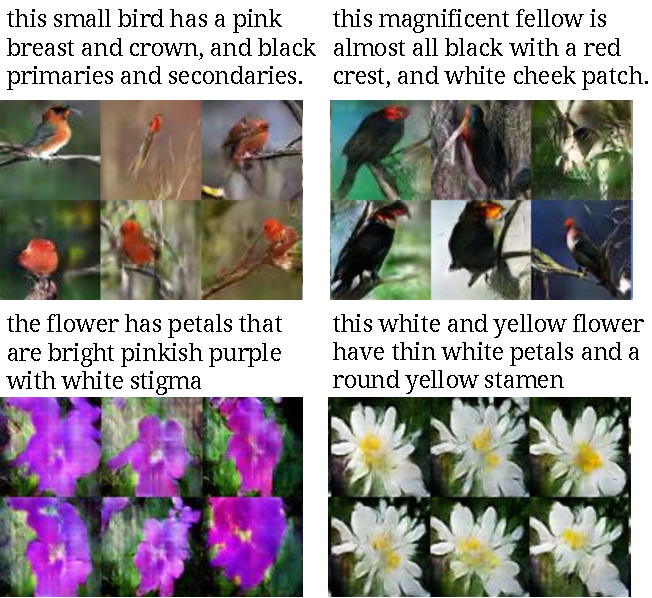
\includegraphics[width=\textwidth]{text2im}
\caption{
Text-to-image synthesis with GANs.
Image reproduced from \citet{reed2016generative}.
}
\label{fig:text2im}
\end{figure}

\begin{figure}
  \centering
  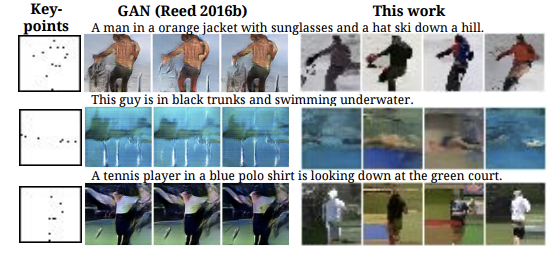
\includegraphics[width=\textwidth]{low_diversity}
  \caption{GANs have low output diversity for text-to-image
    tasks because of the mode collapse problem.
    Image reproduced from \citet{reedgenerating}.
  }
  \label{fig:low_diversity}
\end{figure}

\begin{figure}
  \centering
  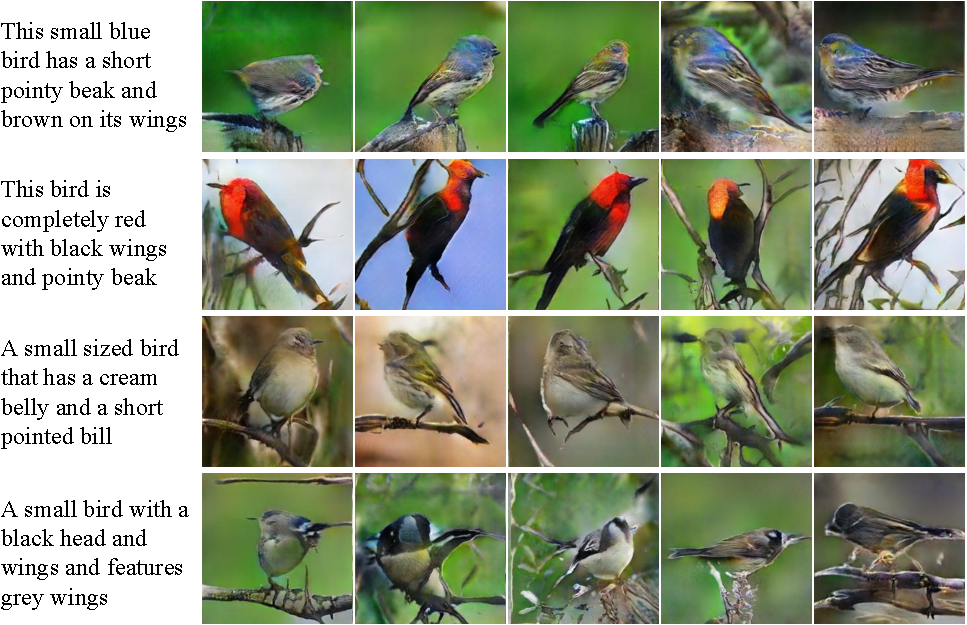
\includegraphics[width=\textwidth]{stackgan}
  \caption{StackGANs are able to achieve higher output
    diversity than other GAN-based text-to-image models.
    Image reproduced from \citet{zhang2016stackgan}.}
    \label{fig:stackgan}
  \end{figure}

The mode collapse problem is probably the most important issue with GANs that
researchers should attempt to address.

One attempt is \newterm{minibatch features} \citep{salimans2016improved}.
The basic idea of minibatch features is to allow the discriminator to compare
an example to a minibatch of generated samples and a minibatch of real samples.
By measuring distances to these other samples in latent spaces, the discriminator
can detect if a sample is unusually similar to other generated samples.
Minibatch features work well.
It is strongly recommended to directly copy the Theano/TensorFlow code released
with the paper that introduced them, since small changes in the definition of the
features result in large reductions in performance.

Minibatch GANs trained on CIFAR-10 obtain excellent results, with most samples
being recognizable as specific CIFAR-10 classes (\figref{fig:minibatch_cifar}).
When trained on $128 \times 128$ ImageNet, few images are recognizable as belonging
to a specific ImageNet class (\figref{fig:minibatch_imagenet}).
Some of the better images are cherry-picked into \figref{fig:cherry}.

\begin{figure}
  \centering
  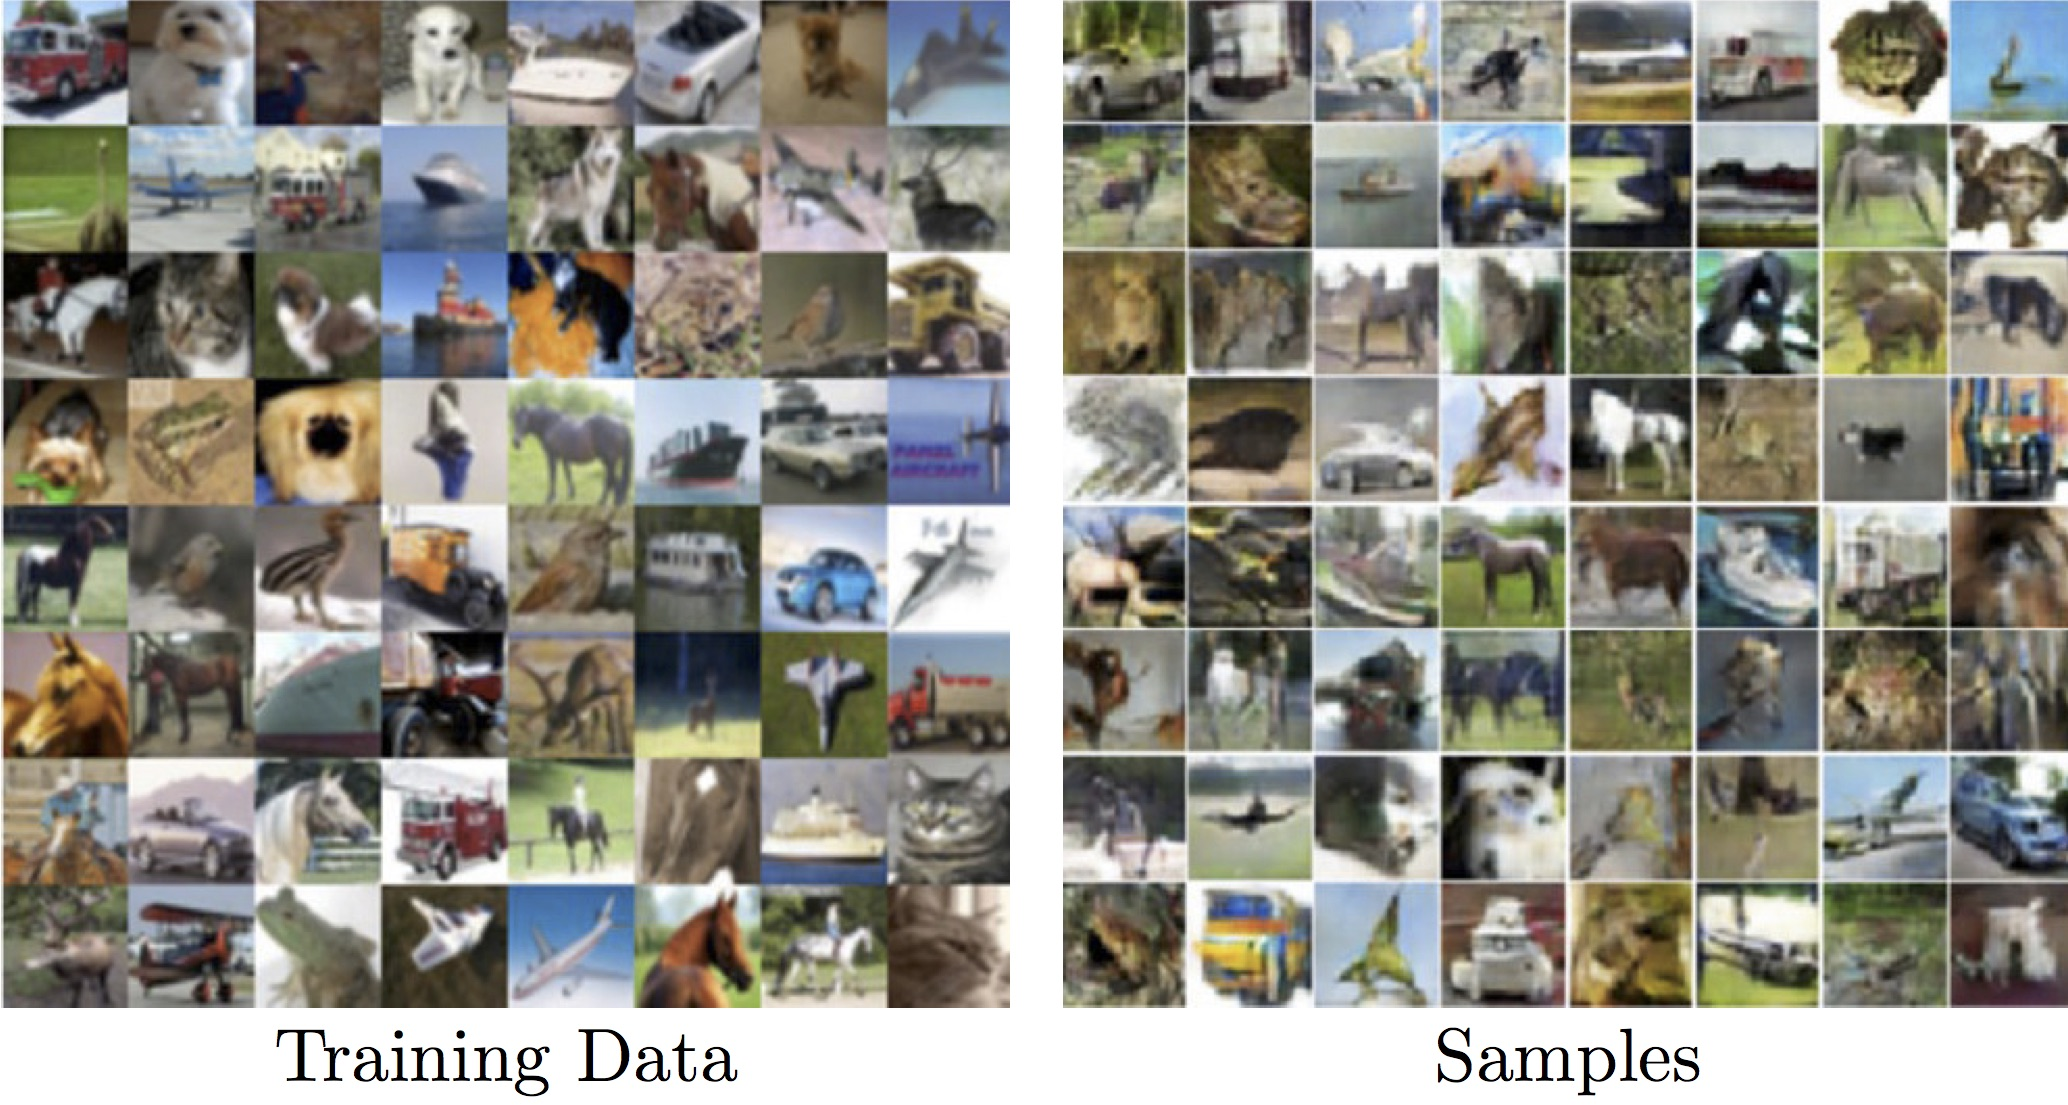
\includegraphics[width=\figwidth]{minibatch_cifar}
  \caption{
    Minibatch GANs trained on CIFAR-10 obtain excellent results, with most samples
    being recognizable as specific CIFAR-10 classes.
    (Note: this model was trained with labels)
  }
  \label{fig:minibatch_cifar}
\end{figure}

\begin{figure}
  \centering
  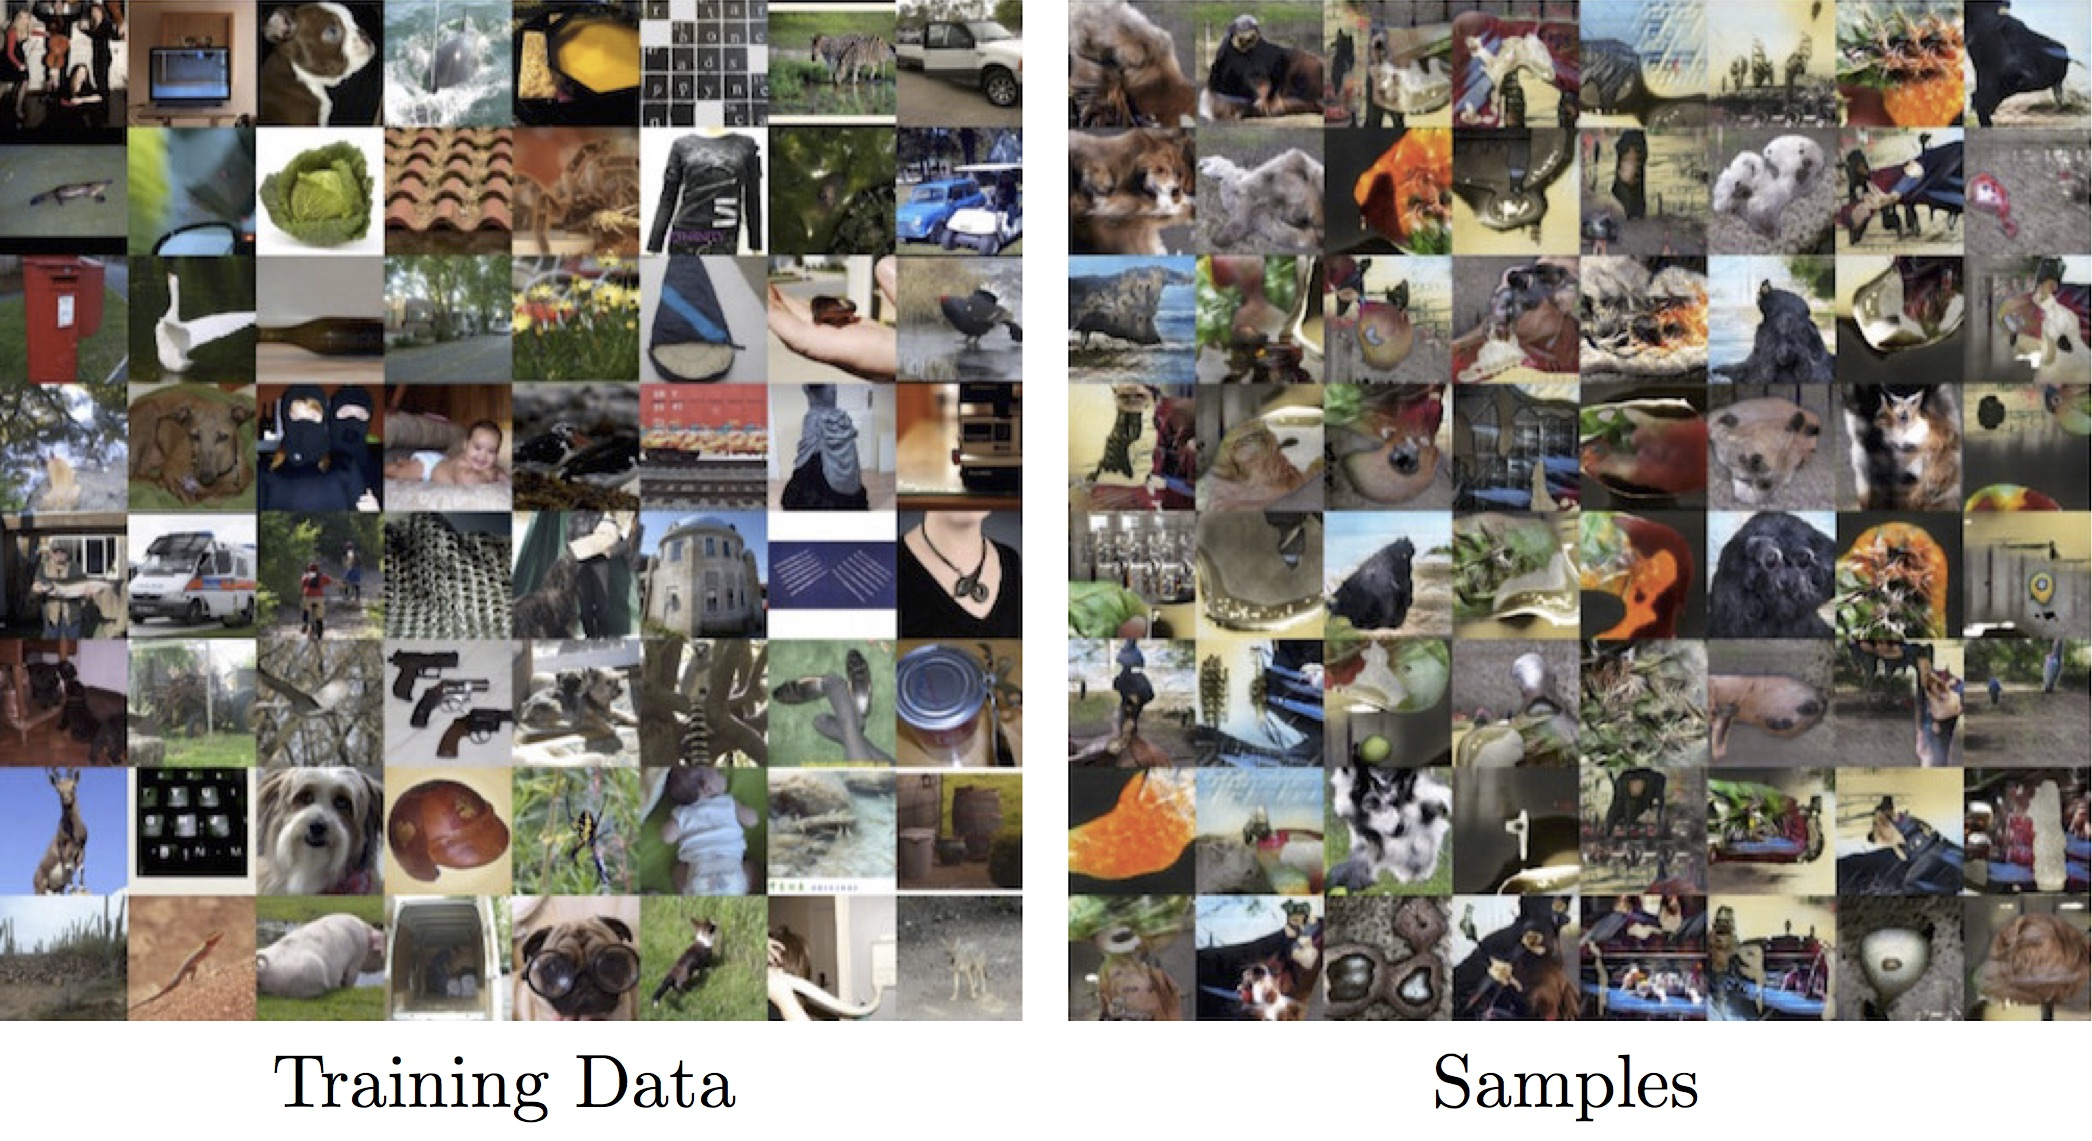
\includegraphics[width=\figwidth]{minibatch_imagenet}
  \caption{
    Minibatch GANS trained with labels on $128 \times 128$ ImageNet produce images
    that are occasionally recognizable as belonging to specific
    classes.
  }
  \label{fig:minibatch_imagenet}
\end{figure}

\begin{figure}
  \centering
  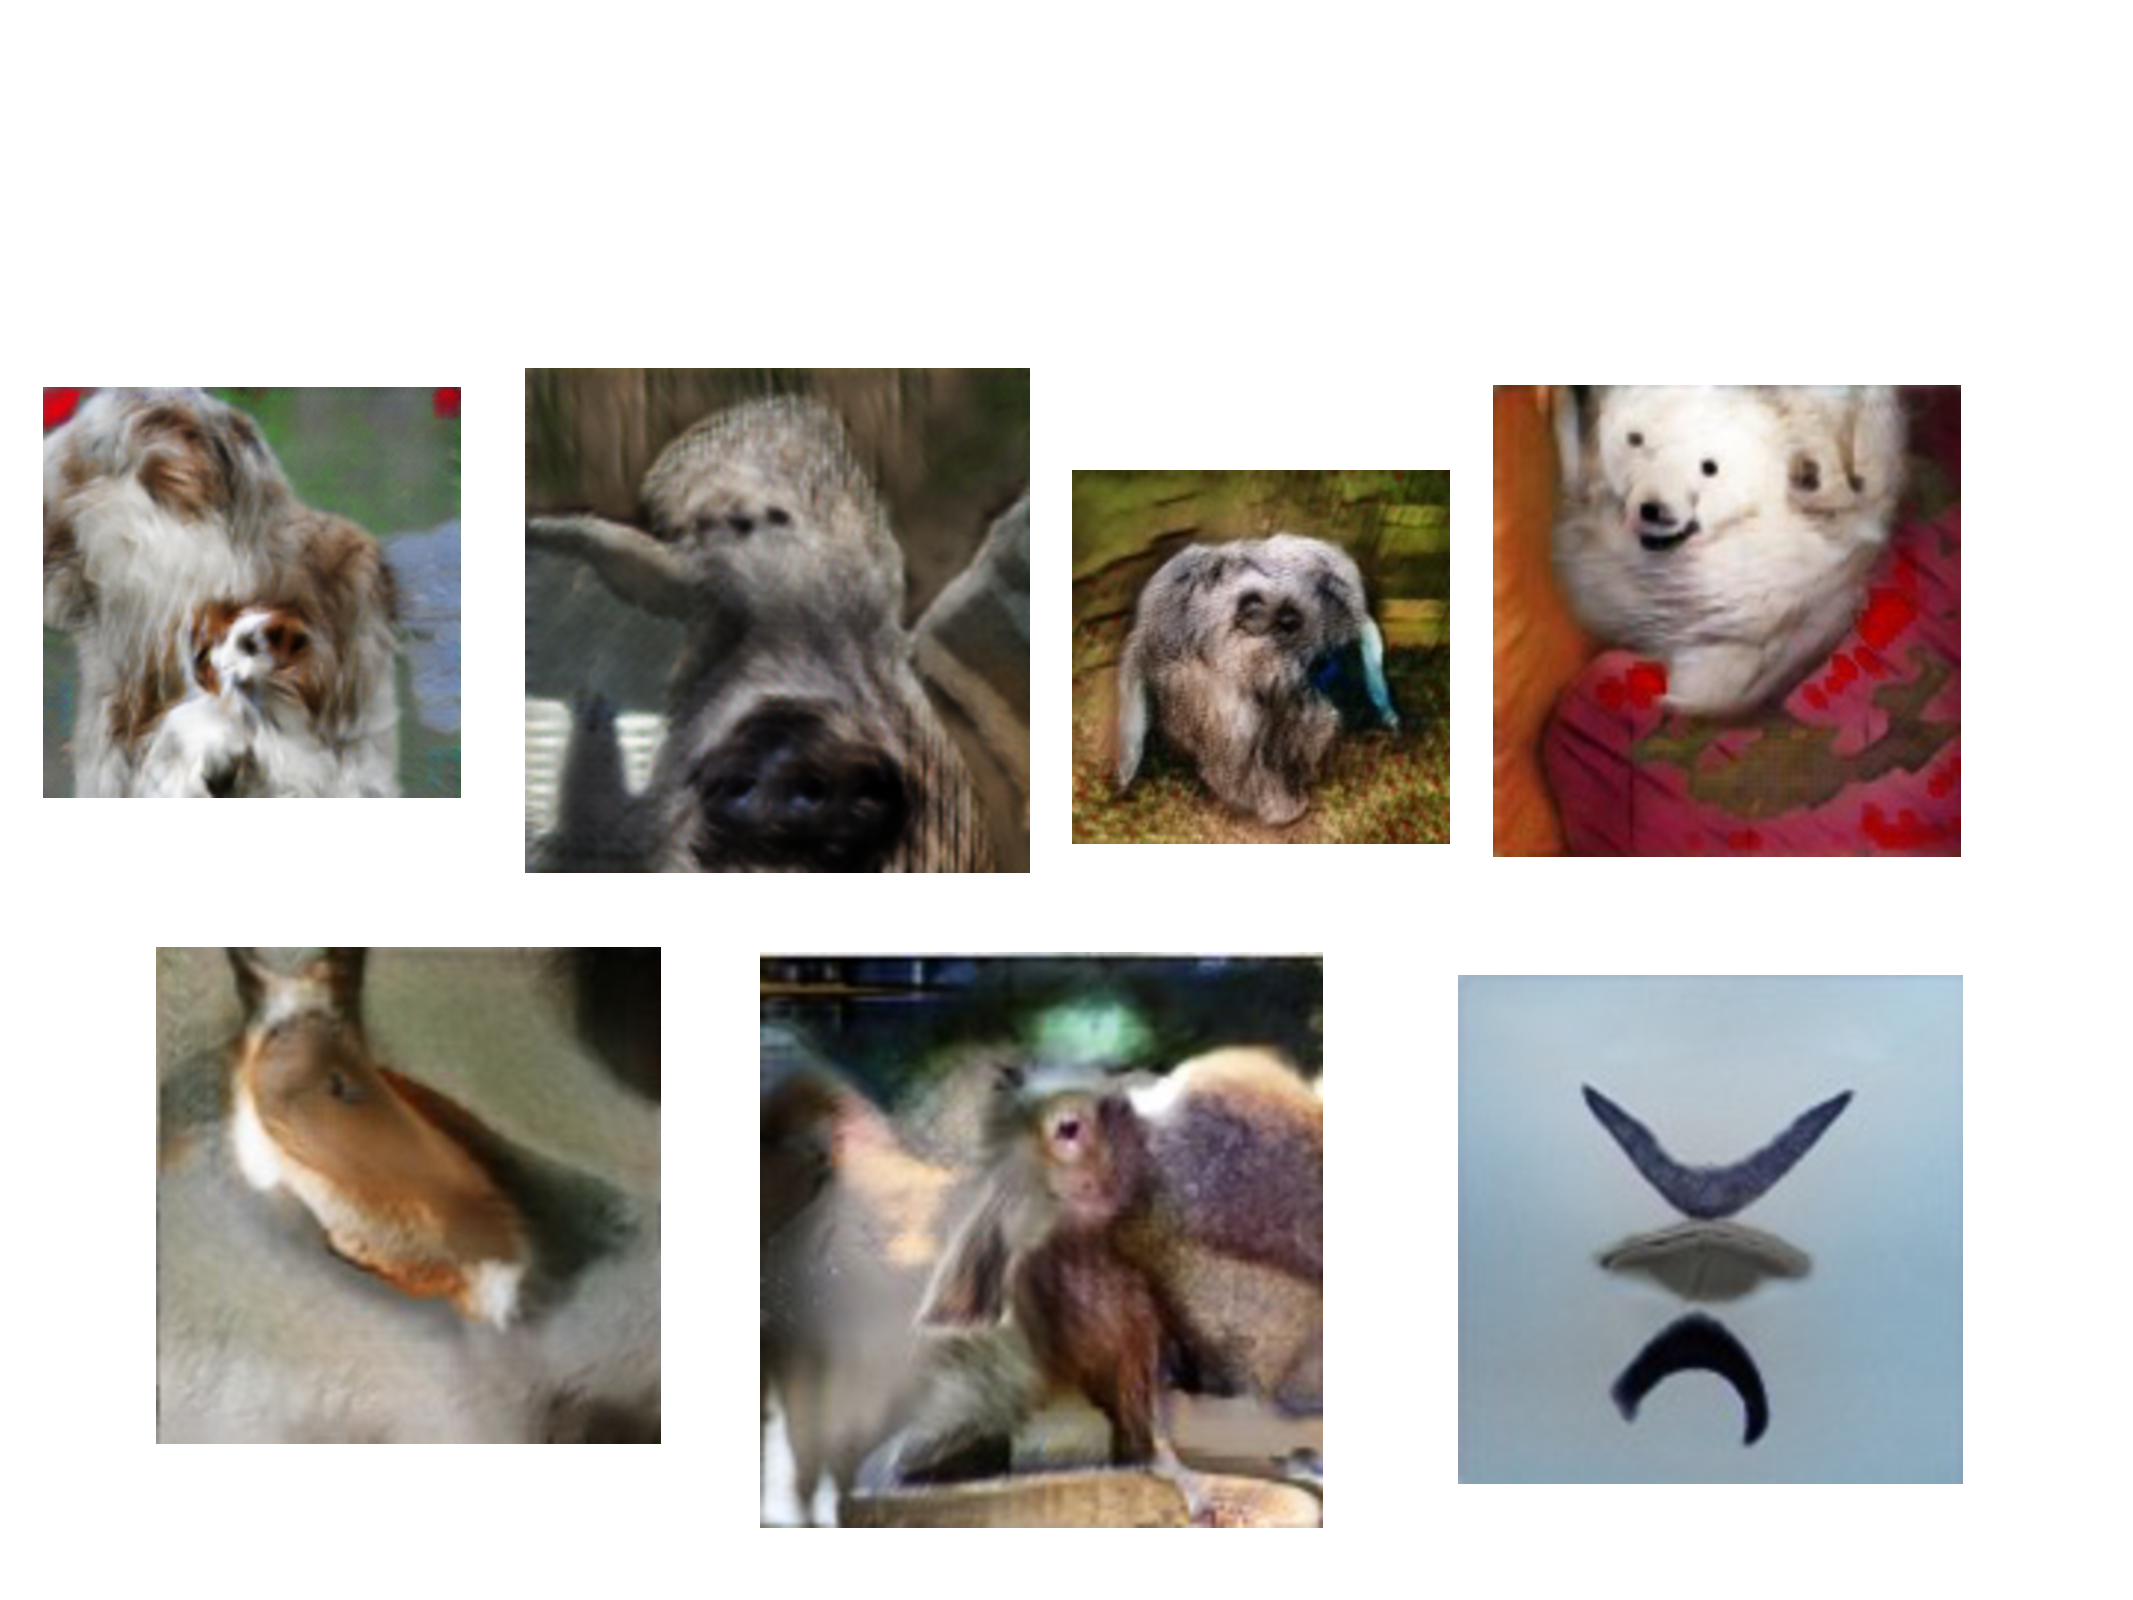
\includegraphics[width=\figwidth]{cherry}
  \caption{
    Minibatch GANs sometimes produce very good images when trained on $128 \times 128$
    ImageNet, as demonstrated by these cherry-picked examples.
  }
  \label{fig:cherry}
\end{figure}

Minibatch GANs have reduced the mode collapse problem enough that other problems, such
as difficulties with counting, perspective, and global structure become the most obvious
defects (\figref{fig:counting}, \figref{fig:perspective}, and \figref{fig:structure},
respectively).
Many of these problems could presumably be resolved by designing better model architectures.


\begin{figure}
  \centering
  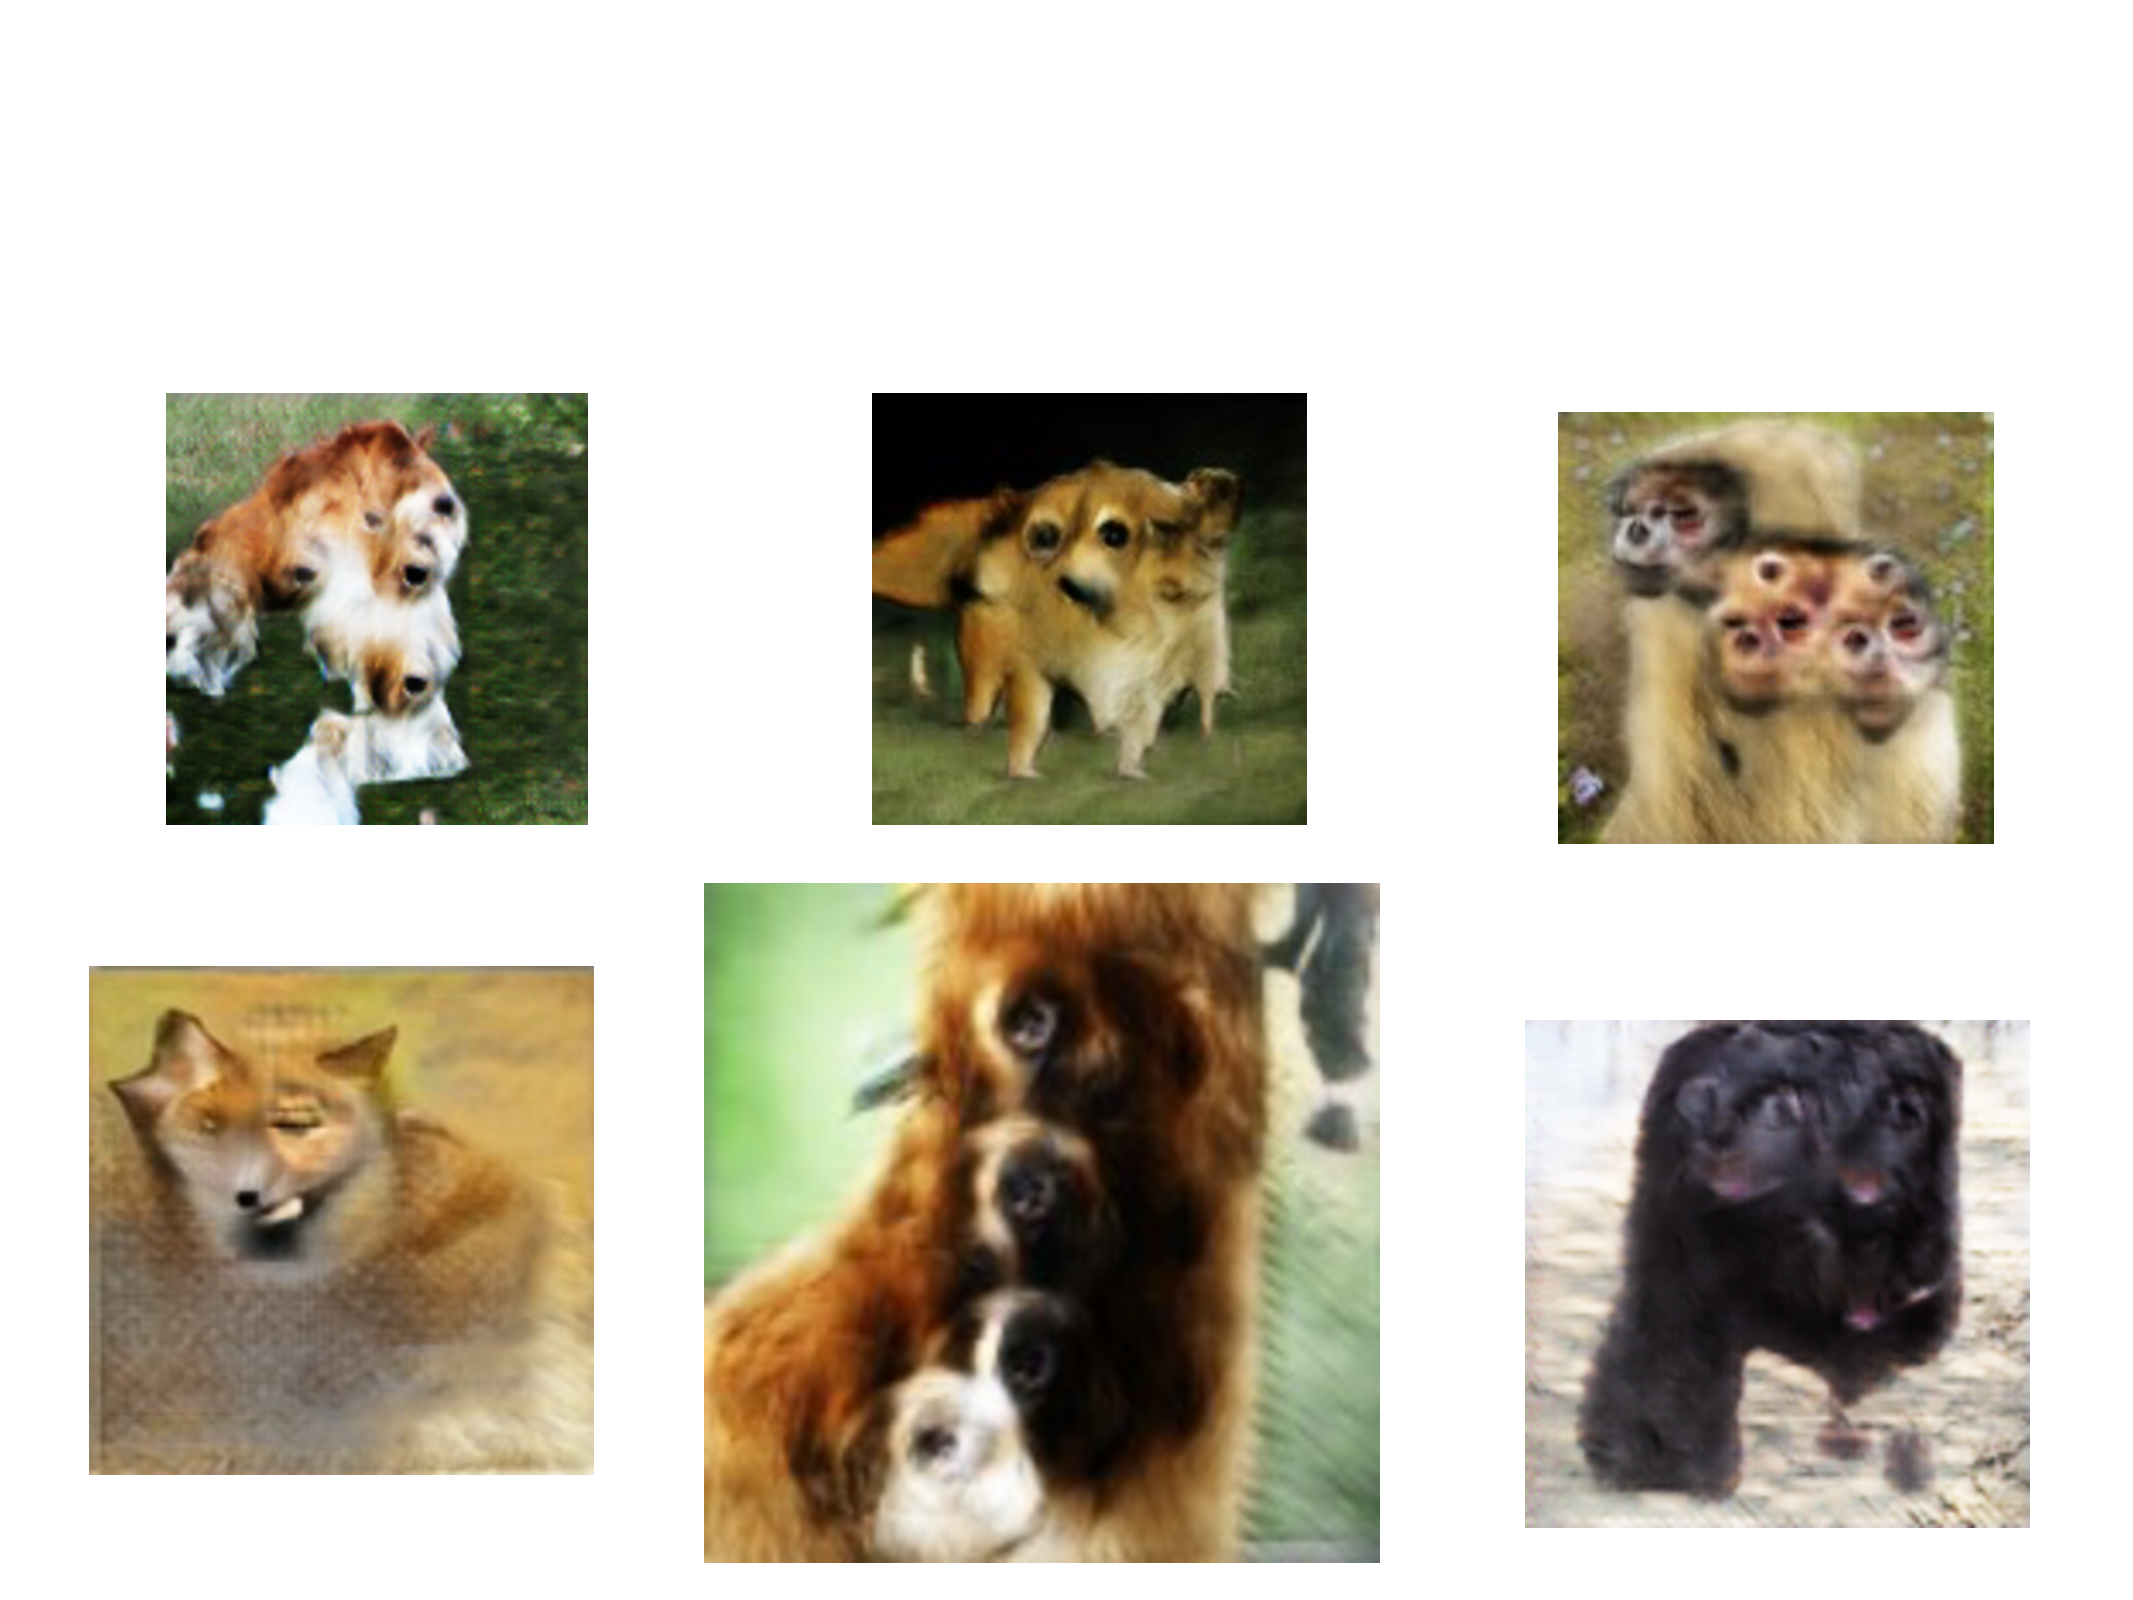
\includegraphics[width=\figwidth]{counting}
  \caption{
    GANs on $128\times 128$ ImageNet seem to have trouble with counting, often generating
    animals with the wrong number of body parts.
  }
  \label{fig:counting}
\end{figure}

\begin{figure}
  \centering
  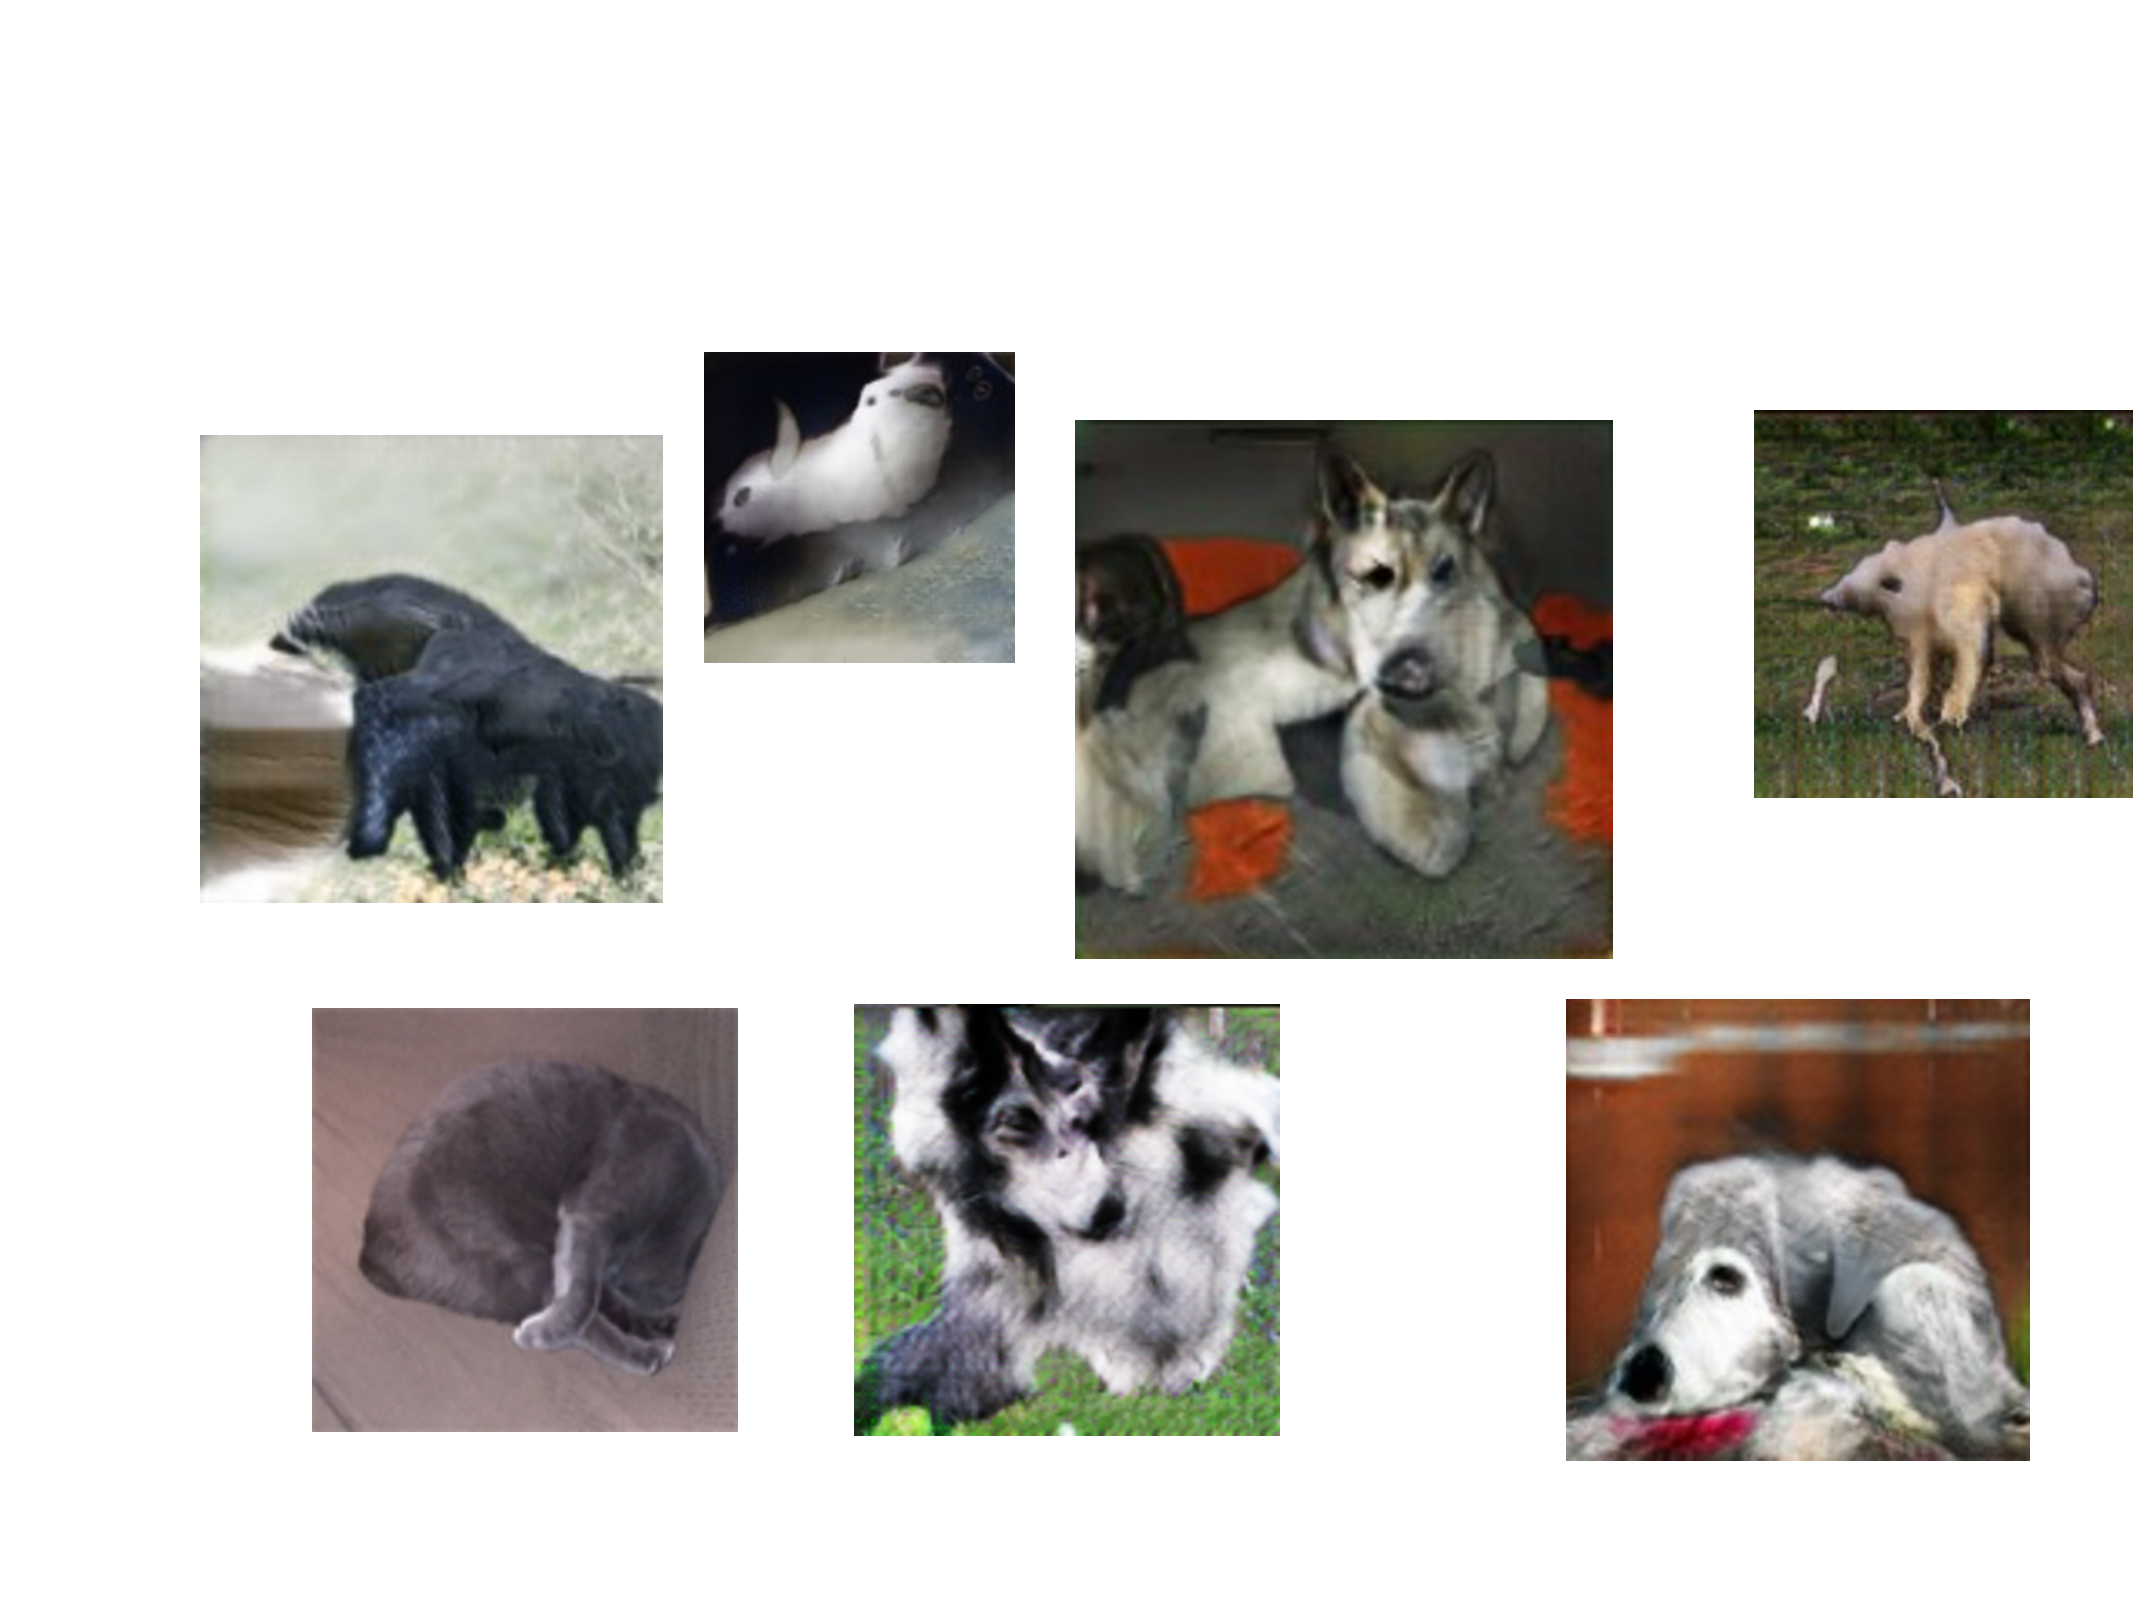
\includegraphics[width=\figwidth]{perspective}
  \caption{
    GANs on $128\times 128$ ImageNet seem to have trouble with the idea of three-dimensional
    perspective, often generating images of objects that are too flat or highly axis-aligned.
    As a test of the reader's discriminator network, one of these images is actually real.
  }
  \label{fig:perspective}
\end{figure}

\begin{figure}
  \centering
  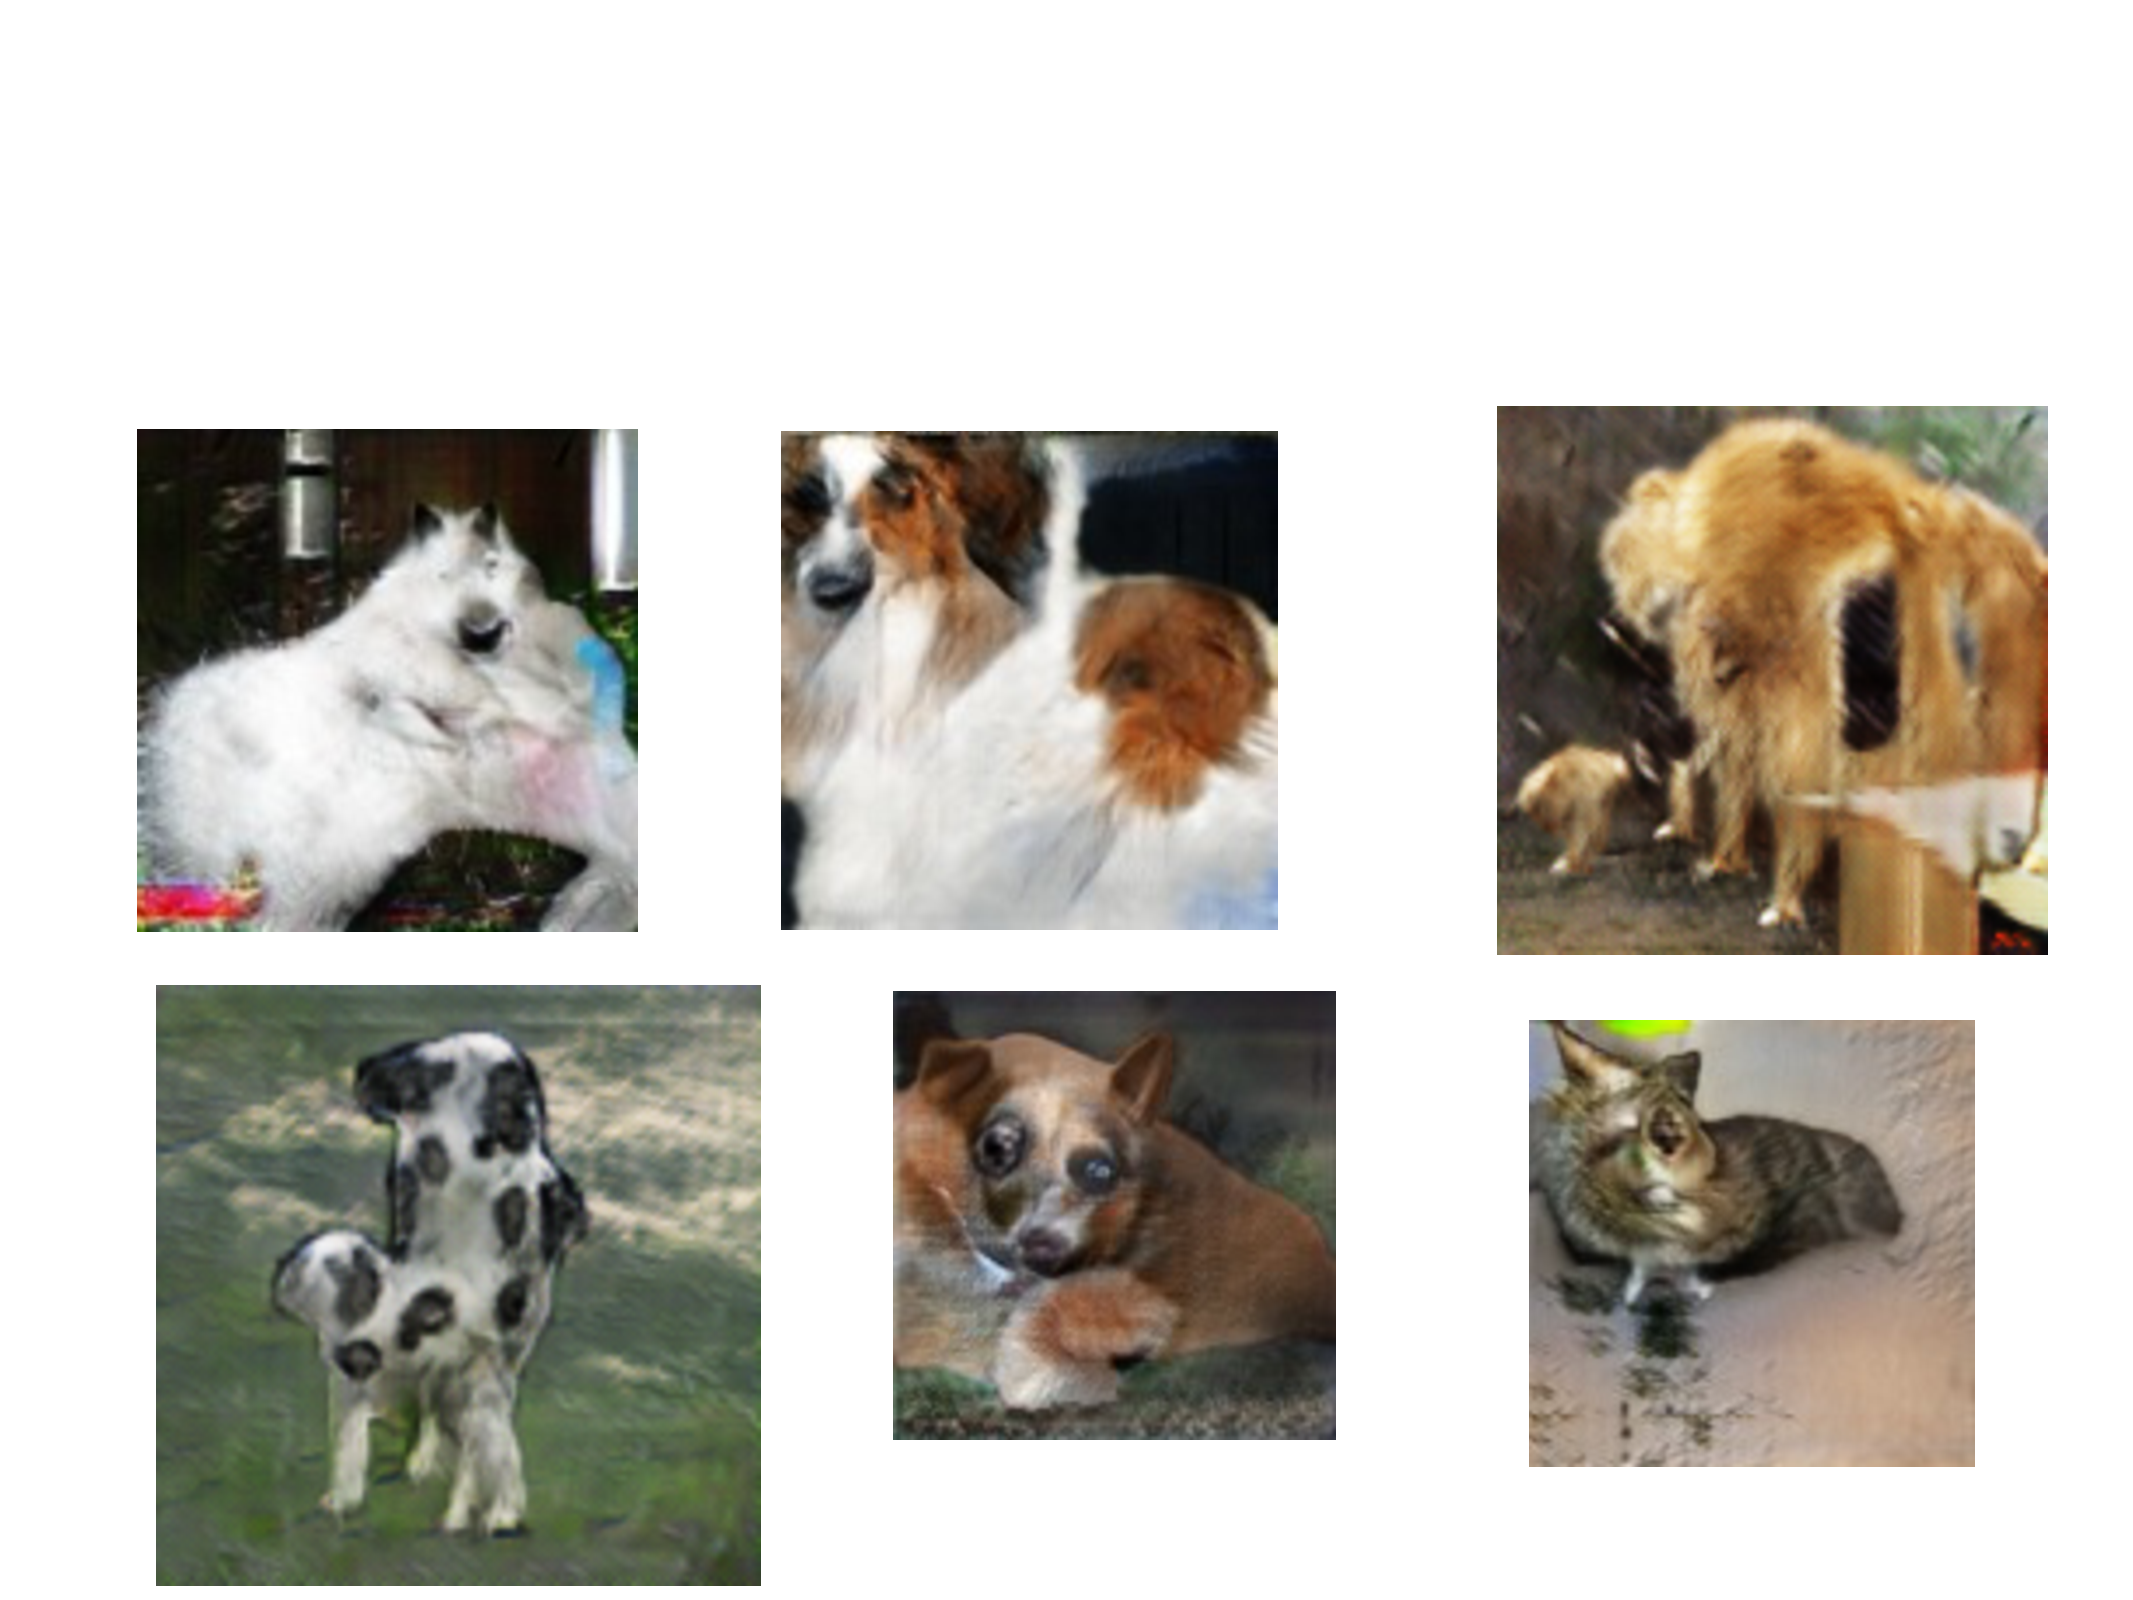
\includegraphics[width=\figwidth]{structure}
  \caption{
    GANs on $128\times 128$ ImageNet seem to have trouble coordinating global structure,
    for example, drawing ``Fallout Cow,'' an animal that has both quadrupedal and bipedal structure.
  }
  \label{fig:structure}
\end{figure}

Another approach to solving the mode collapse problem is \newterm{unrolled GANs} \citep{metz2016unrolled}.
Ideally, we would like to find $G^* = \argmin_G \max_D V(G, D)$.
In practice, when we simultaneously follow the gradient of $V(G, D)$ for both players, we essentially ignore
the $\max$ operation when computing the gradient for $G$.
Really, we should regard $\max_D V(G,D)$ as the cost function for $G$, and we should back-propagate through
the maximization operation.
Various strategies exist for back-propagating through a maximization operation, but many, such as those
based on implicit differentiation, are unstable.
The idea of unrolled GANs is to build a computational graph describing $k$ steps of learning
in the discriminator, then backpropagate through all $k$ of these steps of learning
when computing the gradient on the generator.
Fully maximizing the value function for the discriminator takes tens of thousands of steps,
but \citet{metz2016unrolled} found that unrolling for even small numbers of steps, like 10 or fewer,
can noticeably reduce the mode dropping problem.
This approach has not yet been scaled up to ImageNet.
See \figref{fig:unrolled} for a demonstration of unrolled GANs on a toy problem.

\begin{figure}
  \centering
  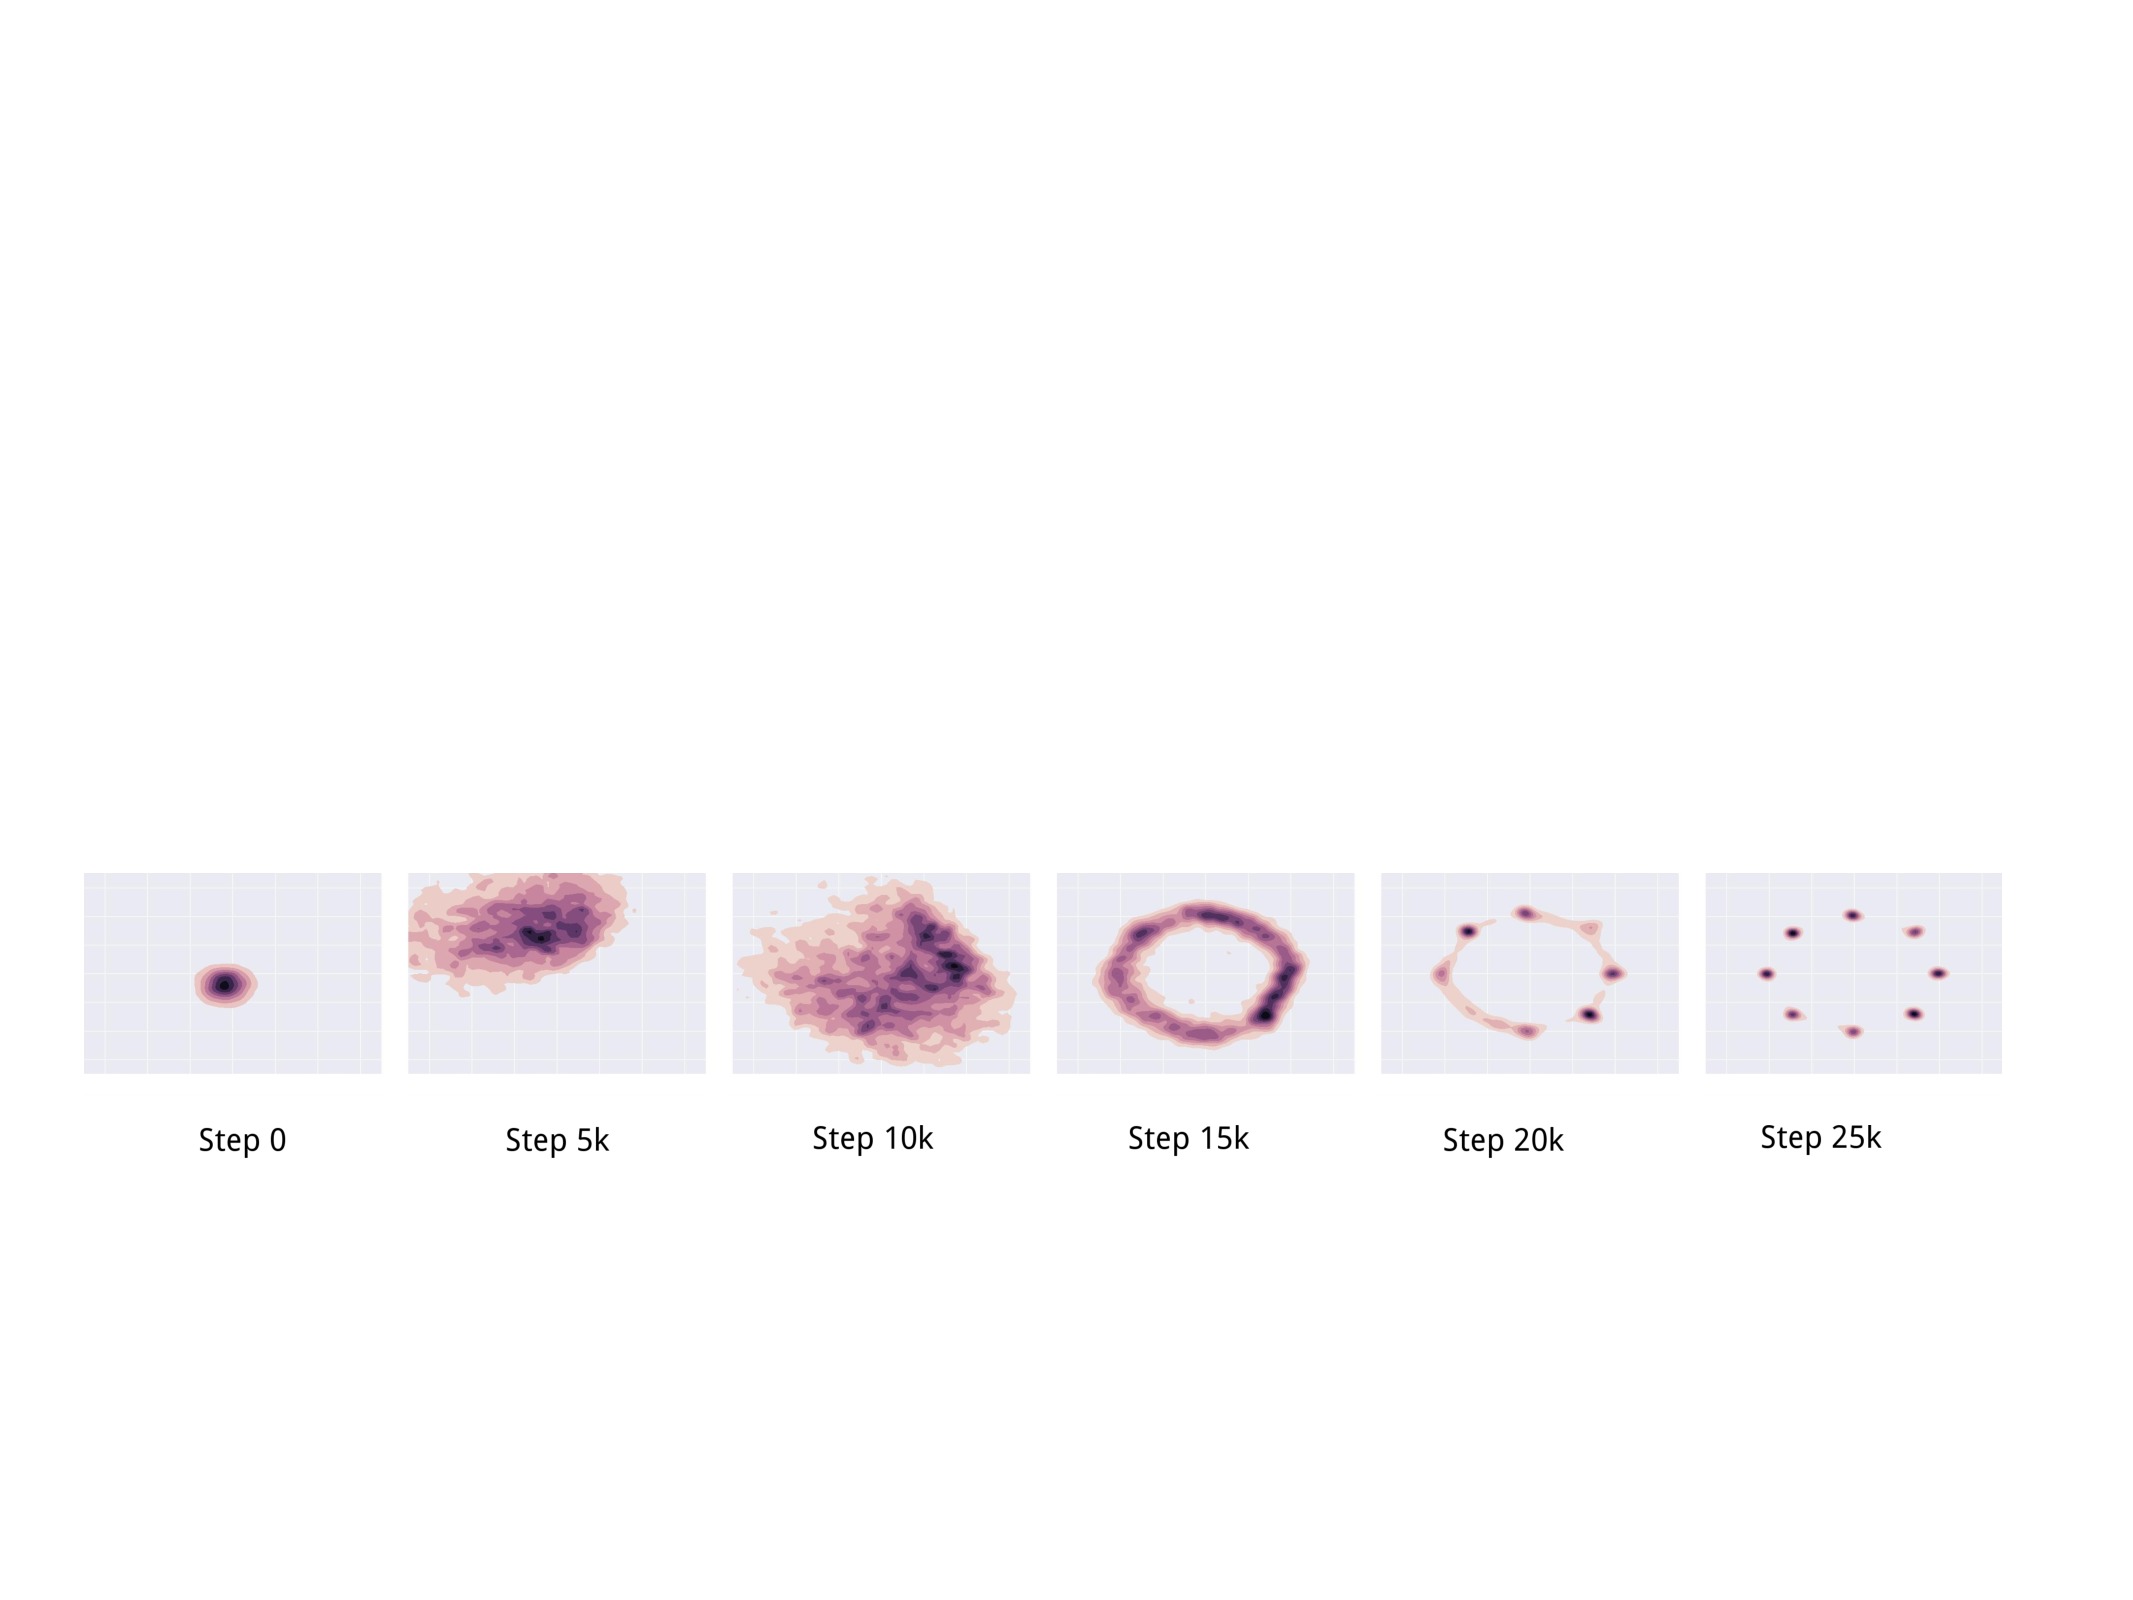
\includegraphics[width=\figwidth]{unrolled}
  \caption{Unrolled GANs are able to fit all of the modes of a mixture of Gaussians
    in a two-dimensional space. Image reproduced from \citet{metz2016unrolled}.
  }
  \label{fig:unrolled}
\end{figure}

\subsubsection{Other games}

If our theory of how to understand whether a continuous, high-dimensional non-convex game 
will converge could be improved, or if we could develop algorithms that converge 
more reliably than simultaneous gradient descent, several application areas besides GANs
would benefit.
Even restricted to just AI research, we find games in many scenarios:
\begin{itemize}
  \item Agents that literally play games, such as AlphaGo \citep{silver2016mastering}.
  \item Machine learning security, where models must resist adversarial examples \citep{Szegedy-ICLR2014,Goodfellow-2015-adversarial}.
  \item Domain adaptation via domain-adversarial learning \citep{ganin2015domain}.
  \item Adversarial mechanisms for preserving privacy \citep{edwards2015censoring}.
  \item Adversarial mechanisms for cryptography \citep{abadi2016learning}.
\end{itemize}
This is by no means an exhaustive list.

\subsection{Evaluation of generative models}

Another highly important research area related to GANs is that it is not clear
how to quantitatively evaluate generative models.
Models that obtain good likelihood can generate bad samples, and models that
generate good samples can have poor likelihood.
There is no clearly justified way to quantitatively score samples.
GANs are somewhat harder to evaluate than other generative models because
it can be difficult to estimate the likelihood for GANs
(but it is possible---see \citet{wu2016quantitative}).
\citet{Theis2015d} describe many of the difficulties with evaluating generative models.

\subsection{Discrete outputs}

The only real requirement imposed on the design of the generator by the GAN framework
is that the generator must be differentiable.
Unfortunately, this means that the generator cannot produce discrete data, such
as one-hot word or character representations.
Removing this limitation is an important research direction that could unlock the
potential of GANs for NLP.
There are at least three obvious ways one could attack this problem:
\begin{enumerate}
  \item Using the REINFORCE algorithm \citep{Williams-1992}.
  \item Using the concrete distribution \citep{maddison2016concrete} or Gumbel-softmax \citep{jang2016categorical}.
  \item Training the generate to sample continuous values that can be decoded to discrete ones (e.g., sampling
    word embeddings directly).
\end{enumerate}

\subsection{Semi-supervised learning}
\label{sec:ssl}

A research area where GANs are already highly successful is the use of generative
models for semi-supervised learning, as proposed but not demonstrated in the original
GAN paper \citep{Goodfellow-et-al-NIPS2014-small}.

GANs have been successfully applied to semi-supervised learning at least since the introduction
of CatGANs \citep{springenberg2015unsupervised}.
Currently, the state of the art in semi-supervised learning on MNIST, SVHN, and CIFAR-10
is obtained by \newterm{feature matching GANs} \citep{salimans2016improved}.
Typically, models are trained on these datasets using 50,000 or more labels,
but feature matching GANs are able to obtain good performance
with very few labels.
They obtain state of the art performance within several categories for different
amounts of labels, ranging from 20 to 8,000.

The basic idea of how to do semi-supervised learning with feature matching GANs
is to turn a classification problem with $n$ classes into a classification problem
with $n+1$ classes, with the additional class corresponding to fake images.
All of the real classes can be summed together to obtain the probability of the
image being real, enabling the use of the classifier as a discriminator within
 the GAN game.
 The real-vs-fake discriminator can be trained even with unlabeled data, which
 is known to be real, and with samples from the generator, which are known to
 be fake.
 The classifier can also be trained to recognize individual real classes on the limited
 amount of real, labeled examples.
 This approach was simultaneously developed by \citet{salimans2016improved}
 and \citet{odena2016semi}. The earlier CatGAN used an $n$ class discriminator
 rather than an $n+1$ class discriminator.

 Future improvements to GANs can presumably be expected to yield further
 improvements to semi-supervised learning.

 \subsection{Using the code}

 GANs learn a representation $\vz$ of the image $\vx$.
 It is already known that this representation can capture useful high-level
 abstract semantic properties of $\vx$, but it can be somewhat difficult
 to make use of this information.

One obstacle to using $\vz$ is that it can be difficult to obtain
$\vz$ given an input $\vx$.
\citet{Goodfellow-et-al-NIPS2014-small} proposed but did not demonstrate
using a second network analogous to the generator to sample from $p(\vz \mid \vx)$,
much as the generator samples from $p(\vx)$.
So far the full version of this idea, using a fully general neural network as the
encoder and sampling from an arbitrarily powerful approximation of $p(\vz \mid \vx)$,
has not been successfully demonstrated,
but
\citet{donahue2016adversarial} demonstrated how to train a deterministic encoder,
and \citet{dumoulin2016adversarially} demonstrated how to train an encoder
network that samples from a Gaussian approximation of the posterior.
Futher research will presumably develop more powerful stochastic encoders.

Another way to make better use of the code is to train the code to be more useful.
InfoGANs \citep{chen2016infogan} regularize some entries in the code vector with
an extra objective function that encourages them to have high mutual information
with $\vx$. Individual entries in the resulting code then correspond to specific
semantic attributes of $\vx$, such as the direction of lighting on an image of
a face.

\subsection{Developing connections to reinforcement learning}
\label{sec:rl_connections}

Researchers have already identified connections between GANs and
actor-critic methods \citep{pfau2016connecting}, inverse reinforcement learning \citep{finn2016connection},
and have applied GANs to imitation learning \citep{ho2016generative}.
These connections to RL will presumably continue to bear fruit, both for GANs
and for RL.

